\documentclass {article}
\usepackage{fullpage}
\usepackage{parskip}
\usepackage{minted}
\usepackage{float}
\usepackage{graphicx}
\usepackage{hyperref}
\hypersetup{
    colorlinks=false,
    linkcolor=blue,
    filecolor=magenta,
    urlcolor=cyan,
}

% biblatex setup
\usepackage[style=numeric,backend=biber,sorting=none]{biblatex} % use biber and order references as they appear
\addbibresource{references.bib} % biblatex file
\emergencystretch=1em % prevent overflow of bib

\DeclareUnicodeCharacter{2500}{-}

\begin{document}

~\vfill
\begin{center}
\Large

CS488 Project Documentation

Title: Kefka --- First-Person Shooter Game Engine

Name: Zac Joffe

Student ID: 20711812

User ID: zmjoffe

\end{center}
\vfill ~\vfill~

\newpage
\tableofcontents

\newpage
\section{Project Outline}
\subsection{Purpose}
To create a 3D environment that can be explored via a first-person perspective.

\subsection{Background \& Motivation}\label{sec:background}
I've always been interested in creating a 3D game engine using OpenGL. First-person shooters have been one of my favourite game genres for well over a decade \footnote{Standout titles of the genre include \textit{Doom}, \textit{Quake}, \textit{Blood}, \textit{Half-Life}, \textit{Portal 2}, and \textit{Metroid Prime}.}. This project is primarily focused on the graphics engine; the gameplay is simple and serves as an interesting context for the implementation of the graphics component. The player controls a character equipped with a firearm in a first-person point of view. The gun can be used to shoot enemies that move in the environment. The player can freely move about the world on the ground-level and look around the environment, just as one would expect from a first-person shooter.

This project was challenging since it employed a wide range of graphics concepts. Nearly all concepts in the pre-ray tracing part of the course were employed, and implementation of each objective was non-trivial. Through this project, I learned how to create a basic 3D game engine which can be used to create a simple first-person shooter. Moreover, I learned a lot about how to architect a game engine. Large parts of the codebase were refactored throughout the development process in order to facilitate new functionality and improve component flexibility. Since much of the ``how'' of implementation was researched during development \footnote{The high-level research I did for the proposal was certainly helpful in implementing the objectives. The ``how'' here refers to the lower level implementation details.}, I made many poor decisions that resulted in a lot of extra work. I believe that is part of the learning process with a project of this scale, and is most certainly expected with my level of experience using OpenGL.

Section~\ref{sec:implementation} documents implementation details of the final code revision. I'll go over my learnings with respect to the designs and potential ways to improve what I've done.

\subsubsection{What is a ``Kefka''?}
The name ``Kefka'' comes from the main antagonist of my favorite game, \href{https://en.wikipedia.org/wiki/Final_Fantasy_VI}{\textit{Final Fantasy VI}}. I've thought of this project as the ``final boss'' of my degree, so this name felt appropriate.

\section{Development}
\subsection{Development Environment}\label{sec:devenv}
The project was primarily developed on my desktop with an AMD 5950x and an Nvidia RTX 3090 running Arch Linux with the latest stable kernel. I briefly tested it on my Framework Laptop with an Intel Core i5 240p (integrated graphics), also running Arch Linux with the latest stable kernel. I also made sure it compiled on the CS488 virtual machine before submission.

Git was used as my version control system. I made an attempt to make each commit represent a feature/bugfix/change so I could leverage \texttt{git bisect} if needed.

The project source is written in C++17, and I (naturally) used Emacs to write all code. The only reason I mention the latter is that my submitted directory includes files \texttt{.projectile} and \texttt{.dir-locals.el}, which are used to help configure my Emacs environment. These can be safely ignored.

\subsection{Project Metadata}
It goes without saying that this project was a lot of work. This subsection is a fun, albeit brief, analysis of the amount of work I put in.

A good place to begin is by showing the number of commits to the master branch:
\begin{minted}[fontsize=\small]{sh}
zac@arch ~/D/C/cs488-project (master) [SIGHUP]> git rev-list --count master
144
\end{minted}

As mentioned in section~\ref{sec:devenv}, most commits contain a single feature/bugfix/change, so the size of each commit varies widely. Using \texttt{git log} and some shell-fu we can see how many lines of code were inserted and deleted over the 144 commits. Note that this is only files in the \texttt{src} directory, as this is where all the C++ source/header files I wrote live. Many more lines were written outside this directory in the form of vertex/fragment shaders, build scripts, and modifications to the CS488 framework.
\begin{minted}[fontsize=\small]{sh}
zac@arch ~/D/C/cs488-project (master)> git log --author="Zac Joffe" --pretty=tformat: --numstat -- src/ | awk '{ inserted+=$1; deleted+=$2 } END { print "Lines inserted: " inserted, "Lines deleted: " deleted }'
Lines inserted: 5395 Lines deleted: 2826
\end{minted}

I wrote a lot of code! And deleted a lot of it too. As mentioned in section~\ref{sec:background}, I had to refactor and rearchitect quite often throughout development, which explains the numbers above.

Using the \href{https://github.com/boyter/scc}\texttt{scc} tool, we can see some interesting metadata about the C++ source/header files in the \texttt{src} directory:
\begin{minted}[fontsize=\small]{sh}
zac@arch ~/D/C/c/src (master)> scc .
───────────────────────────────────────────────────────────────────────────────
Language                 Files     Lines   Blanks  Comments     Code Complexity
───────────────────────────────────────────────────────────────────────────────
C Header                    20       894      200        17      677          0
C++                         18      1675      318        78     1279        145
Emacs Lisp                   1         1        0         0        1          0
───────────────────────────────────────────────────────────────────────────────
Total                       39      2570      518        95     1957        145
───────────────────────────────────────────────────────────────────────────────
Estimated Cost to Develop (organic) \$54,672
Estimated Schedule Effort (organic) 4.56 months
Estimated People Required (organic) 1.07
───────────────────────────────────────────────────────────────────────────────
Processed 73866 bytes, 0.074 megabytes (SI)
───────────────────────────────────────────────────────────────────────────────
\end{minted}
I'm not quite sure how the ``Cost to Develop'' metric is measured, though I must say it's a humbling number.

\section{Manual}\label{sec:manual}
\subsection{Building \& Running}
The submitted \texttt{cs488-project.zip} file includes the \texttt{cs488-project} directory, which has a similar structure to the \texttt{cs488} directory given at the start of the term. The \texttt{cs488-project} directory will be referred to as the ``root'' or ``project root'' directory. \texttt A detailed explanation of the project structure can be found in section~\ref{sec:structure}. The build system was simplified to use a single \texttt{premake4} build script.

To build the code, run the \texttt{premake4} script from the root directory as follows:
\begin{minted}[fontsize=\small]{sh}
$ premake4 gmake && make
\end{minted}

This will compile and link all the necessary libraries and project files. The resulting binary, \texttt{fps}, is outputted in the current working directory. All libraries are statically linked, but the asset paths are hardcoded. Therefore, the binary must be ran with the project root the current working directory. Running the binary is done as follows:
\begin{minted}[fontsize=\small]{sh}
$ ./fps
\end{minted}

There are no command line arguments (or, rather, any provided arguments will be ignored). The game will launch in a window with a resolution of \texttt{1024 x 768}, and is not designed to be resized \footnote{Resizing the window in the main menu before starting the game will make the game render correctly at the new resolution. Resizing the window when playing the game will cause distortions.}. The name of the window is \texttt{CS488\_Project\_FPS}.

\subsection{Main Menu}
When the game starts, the player is presented with the main menu, which is shown in figure~\ref{fig:mainmenu}.

\begin{figure}[H]
  \begin{center}
  \includegraphics[width=\textwidth]{main\_menu.png}
  \end{center}
  \caption{Screenshot of main menu}\label{fig:mainmenu}
\end{figure}

The main menu contains two buttons: ``Start Game'' and ``Options''. The ``Start Game'' button, as one might expect, exits the main menu and starts the game. The ``Options'' button opens a submenu containing a number of widgets to customize the game experience. A screenshot of the options submenu is shown in figure~\ref{fig:optionsmenu}.
\begin{figure}[H]
  \begin{center}
  \includegraphics[width=\textwidth]{options\_menu.png}
  \end{center}
  \caption{Screenshot of options submenu with default game parameters}\label{fig:optionsmenu}
\end{figure}

The ``World Size'' slider tweaks the size of the $N x N$ world of the game on the horizontal ($x-z$) plane. See section~\ref{sec:modelscene} for more details about game world. This slider lets you pick integers in the range of $[20, 75]$.

The ``Num Enemies'' slider tweaks the number of enemies that spawn in the world. This slider lets you pick integers in the range of $[3, 10]$.

The ``Floor Texture'' list box selects the texture that is used to map onto the floor of the game world. Similarly, the ``Wall Texture'' and ``Enemy Texture''\footnote{The ``Mayahem'' family of textures are different stones. The name is a reference to the first level in \href{https://en.wikipedia.org/wiki/Banjo-Tooie}{\textit{Banjo-Tooie}}, \textit{Mayahem Temple}, where the titular hero Banjo transforms into a \href{https://banjokazooie.fandom.com/wiki/Stony_Banjo}{``Stony''} to play in a kickball tournament.} list boxes select the texture used to map onto the walls and enemies in the world, respectively. The ``Skybox'' list box selects the set of textures used to form the skybox.

The ``Back to Main Menu'' button goes back to the parent main menu. Note that parameters are automatically saved after being tweaked, so starting the game from the main menu will start it with the parameters outlined in the options submenu.

At any point in any menu, the \texttt{escape} key can be pressed to close the window. Additionally, the \texttt{s} key will start the game in either menu.

\subsection{The Game}\label{sec:game}
The game consists of an $N x N$ world that the player spawns in. Players are free to move within the $N x N$ world, though they cannot move outside of the world boundaries defined by the walls. Enemies move spawn in random locations and move around the world randomly. If a player shoots an enemy, they will fall to the ground and stop moving. Note that there are no strict objectives to the game, and thus no win or lose states. A screenshot of the game is shown in figure~\ref{fig:game}.
\begin{figure}[H]
  \begin{center}
  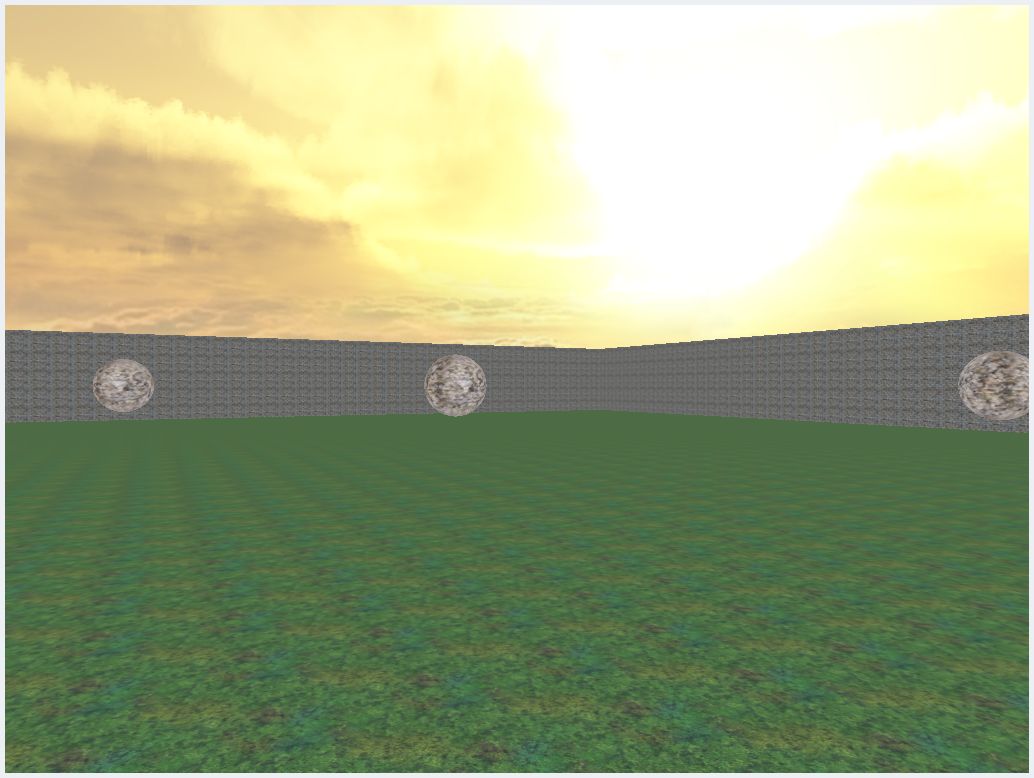
\includegraphics[width=\textwidth]{game.png}
  \end{center}\caption{Screenshot of game with default game parameters}\label{fig:game}
\end{figure}

\subsubsection{Game Controls}\label{sec:controls}
The game is controlled using the mouse and keyboard. If you've played a first-person shooter in the last 25 years, the controls should feel familiar and intuitive. An outline of the game controls is as follows:
\begin{itemize}
  \item \texttt{w}: Move forward.
  \item \texttt{a}: Move (strafe) left.
  \item \texttt{s}: Move back.
  \item \texttt{d}: Move (strafe) right.
  \item \texttt{space}: Jump.
  \item \texttt{left shift}: Hold to spring.
  \item \texttt{r}: Respawn all enemies.
  \item \texttt{escape}: Close the window.
  \item \texttt{left mouse button}: Shoot gun.
\end{itemize}

The mouse is used to look around the world. That is, moving the mouse in a direction moves rotates the camera in that direction accordingly.

\section{Implementation}\label{sec:implementation}
% with an attempt to use reasonably modern C++ techniques.

\subsection{Project Structure}\label{sec:structure}
% TODO talk about started code, premake script, etc.

\subsection{Objective 1: Modeling the Scene}\label{sec:modelscene}
This objective is about modeling the area that the player moves around in. This will be a simple scene with a flat, rectangular floor and four surrounding walls.

% TODO talk about scene, containing tiles, enemies, etc.

\subsection{Objective 2: UI}\label{sec:ui}
The game will launch in a main menu that is visually distinct from normal gameplay. The menu will have a button that lets players start the game. Implementation of this feature can be done with a finite state machine containing two states --- one for the game, and one for the main menu. This state machine can be implemented with the State design pattern by leveraging polymorphic rendering methods, as described in the Gang of Four design patterns chapter of \textit{Game Programming Patterns}~\cite{state}.

\subsection{Objective 3: Texture Mapping}
Texture mapping will be employed to give surfaces more detail and realistic appearances. The approach to implementing texture mapping in OpenGL largely the same as that first described by Blinn and Newell~\cite{texture}. 2D texture rasters are loaded from disk onto the GPU. Texture coordinates $u, v$ are passed as input to the vertex shader, which outputs it to the fragment shader. The fragment shader uses the input texture coordinates to determine the fragment's color. With the \texttt{GL\_LINEAR} texture filtering option, OpenGL performs bilinear interpolation of the texels surrounding texture coordinates to calculate the color.

% https://www.opengl-tutorial.org/beginners-tutorials/tutorial-5-a-textured-cube
% https://learnopengl.com/Getting-started/Textures
% https://www.youtube.com/watch?v=u-00hjlfMKc
% NOTE the uv values are for each vertex, and I should be able to hardcode them (or calculate them) on the cpu

\subsection{Objective 4: Particle System}
%Particle system.
A particle system will be implemented to model muzzle flash of the gun after gun it is fired. An implementation of particle systems is outlined in \textit{Learn OpenGL: Learn Modern OpenGL Graphics Programming in a Step-by-step Fashion.}~\cite{learnopengl}. Particles are implemented using a particle emitter, which spawns a myriad of particles stochastically in a region with given colors, lifetimes, and velocities. Particles are killed after reaching a certain height in the world or after a set amount of time.

% https://learnopengl.com/In-Practice/2D-Game/Particles
% https://www.opengl-tutorial.org/intermediate-tutorials/billboards-particles/particles-instancing/

\subsection{Objective 5: Synchronized Sound}
Sounds will be played to give feedback for specific player actions. For instance, the action of firing the gun may be accompanied by a synchronized gunshot noise. These sounds are implemented as sound files on disk that are loaded into the game engine. Many C++ high-level audio libraries could be utilized to play these sounds, such as \href{https://github.com/libsdl-org/SDL\_mixer}{\texttt{SDL\_mixer}} and \href{https://solhsa.com/soloud/}{\texttt{SoLoud}}.

\subsection{Objective 6: Static Collision Detection}
Static collision detection will be employed to prevent the player from moving out of the bounds defined by scene. The player's location will be surrounded by an invisible axis-aligned bounding box (AABB). The size of this box will be make to enclose the imaginary player character model. All collidable objects will have an AABB. Upon player input for movement, the updated position of the player will be calculated. Then, prior to rendering the update on said frame, every collidable object in the scene will be tested for collision with the player by testing for intersection of AABBs. If a collision occurs, player locations are not updated to the updated value that was calculated prior to the collision tests.

\subsection{Objective 7: Dynamic Collision Detection}
Enemies will move around the scene dynamically, thus a dynamic collision detection algorithm is necessary to determine if a bullet shot by the player hits the enemy. The implementation of this will be done with hitscanning, which is very similar to the ray casting algorithm as described in the ray tracing chapter of \textit{Fundamentals of Computer Graphics}~\cite{rtbook}. When the player shoots their gun, a ray will be casted from the camera in the direction of the gunshot. Each enemy will have an AABB, similar to the static scene geometry in objective 6, which will be used to compute ray-enemy intersection. The nearest enemy hit will then take damage in some visible way.

% all enemies (contained in a list) will be tested for collision
% simplify calculations by using an AABB for enemy

\subsection{Objective 8: Physics Engine}
The physics engine will govern player movement with its simulation of friction and gravity. When a player releases a movement key, friction will cause the character to slow to a stop rather than stopping instantaneously. In classical mechanics, friction can be modeled as a function of material properties (coefficient of friction) and the normal force of the moving object. This model is simplified to a function that reduces the magnitude of the velocity linearly to 0 at a convincing rate.

Gravity simulation will allow for realistic jumping mechanics. In classical mechanics, gravity (on earth) is represented as a constant force acting down on an object at a rate proportional to its mass. This model is simplified by ignoring the mass of the player (or rather setting the gravitation acceleration to account for the player's mass accordingly). Upon jumping, the player's height will increase by some initial velocity. The force of gravity will cause this velocity to decrease over time by a constant acceleration value. This will cause the player to rise and fall in the same way one would if they were to jump in the real world.

\subsection{Objective 9: Shadow Mapping}
I did not have time to finish this objective. The work I did is committed in the \texttt{shadow-mapping} branch in the submitted code. The branch is based on a mostly up-to-date revision to the master branch. I'll briefly go over the work I did and how I would have finished implementing it if given the time.

TODO talk about it

% Shadows are implemented in the world using shadow mapping. This algorithm was first described by Williams in 1978 \cite{shadowmapping}, and involves a two-pass rendered where the world is rendered from the light's point of view, then rendered from the camera's point of view. The second rendering pass uses z-buffer values computed from the first rendering pass to determine if a pixel is visible from the light source, and draws shadows accordingly.

\subsection{Objective 10: Keyframe Animation}
I did not attempt this objective.


\newpage
\printbibliography[heading=bibintoc, title={References}] % https://tex.stackexchange.com/a/279977

\newpage
\appendix
\section{Objectives}\label{sec:objectives}
\begin{enumerate}
    \item[\textbf{1:}]
    Model the scene for the player to move around in.

    \item[\textbf{2:}]
    Main menu user interface that the player interacts with to start the game.

    \item[\textbf{3:}]
    Texture mapping.

    \item[\textbf{4:}]
    Particle system.

    \item[\textbf{5:}]
    Synchronized sound corresponding to player actions.

    \item[\textbf{6:}]
    Static collision detection of surrounding environment.

    \item[\textbf{7:}]
    Dynamic collision detection of bullets fired by the player with enemies in the environment.

    \item[\textbf{8:}]
    Physics engine with friction and gravity.

    \item[\textbf{9:}]
    Shadows using shadow mapping.

    \item[\textbf{10:}]
    Keyframe animation using linear interpolation.
\end{enumerate}


\end{document}
